\documentclass[a4paper,12pt, notitlepage]{article}

\usepackage[top=25mm,bottom=25mm,left=25mm,right=25mm]{geometry}

\usepackage{amsmath} 
\usepackage{graphicx}
\usepackage{epstopdf}
\usepackage{url}
\usepackage{setspace} 
\setstretch{1.44}
\setlength{\columnsep}{6mm}
\usepackage{titlesec}
\titleformat{\section}{\bfseries\large\scshape\filcenter}{\thesection}{1em}{}
\titleformat{\subsection}{\bfseries\normalsize\scshape\filcenter}{\thesubsection}{1em}{}

% Following change makes the caption size footnotesize From: http://rorasa.wordpress.com/2010/01/13/instant-latex-command-for-small-figure-and-table-caption/  

\renewcommand{\abstractname}{}    % clear the title
\newcommand{\captionfonts}{\footnotesize}
\renewcommand\thesection{\Roman{section}.}
\renewcommand\thesubsection{\Alph{subsection}.}

\makeatletter
\long\def\@makecaption#1#2{
  \vskip\abovecaptionskip
  \sbox\@tempboxa{{\captionfonts #1: #2}}%
  \ifdim \wd\@tempboxa >\hsize
    {\captionfonts #1: #2\par}
  \else
    \hbox to\hsize{\hfil\box\@tempboxa\hfil}%
  \fi
  \vskip\belowcaptionskip}

\renewcommand\p@subsection{\thesection}
    
\makeatother


\begin{document}
%%%%%%%%%%%%%%%%%%%%%%%%%%%%%%%%%%%%%%%%%%%%%%%%%%%%%%%%%%%%%%%%%%%%%%%%%%%%%%%%%%%%
\title{\textbf{\large{Final Year Physics Project – Final Report}}}

\author{\normalsize{University Registration/ Library Card No. (Do not put your name here)} \\
        \small\textit{
        Department of Physics, University of Warwick,
        Coventry CV4 7AL, United Kingdom}}
\date{}


\maketitle 
\vspace{-10mm}

\begin{abstract} 
\noindent
This is where you should put your abstract. You should try and make your abstract as concise as possible giving the general aim of the investigation as well as the major results. The abstract should be around 50 - 100 words and be able to be read in isolation.  
\end{abstract}
\vspace{6mm}
 

%%%%%%%%%%%%%%%%%%%%%%%%%%%%%%%%%%%%%%%%%%%%%%%%%%%%%%%%%%%%%%%%%%%%%%%%%%%%%%%%%%%%
\section{About this Document}
This file provides a basic \LaTeX\ template for the Final Report required for PX402 and PX319 at the University of Warwick. Please feel free to extend the functionality of this template by adding additional packages and settings. However, any definitions regarding the size, font size, margin sizes, etc. should not be changed. However, you can use either single or two column format. The single column format can be achieve by deleting ``twocolumn'' from the first line of the .tex file.

In the following sections I will try give some of the basics of \LaTeX\ that you're likely to use during writing your report. Whenever I refer to something or you find something you want to use, simply refer to that place in the .tex file. However, there is also a wealth of good resources on the web that can also be used so please feel free to refer to them instead.

One final note, this .tex file contains figures, so you might have a few errors when compiling it as you won't have the  picture files in your directory.  

This template was original created by Dirk O. Gericke (Warwick) in 2013 and has been edited by Daniel Brunt (2015). 


%%%%%%%%%%%%%%%%%%%%%%%%%%%%%%%%%%%%%%%%%%%%%%%%%%%%%%%%%%%%%%%%%%%%%%%%%%%%%%%%%%%%
\section{Introduction}
The introduction is where you will discuss the overall aims and objectives of your investigation as well giving a general picture of why it is important. You will most likely have to link it back to previously published literature like  \cite{Paper_1} or you may also have to refer to multiple papers \cite{Paper_1, Paper_2, Paper_3}. Please note you'll have to compile the document twice before the citations appear. The references should be to literature journals or published books. References from websites should only be used sparingly and if possible the information from websites should be traced back to the original source. 


%%%%%%%%%%%%%%%%%%%%%%%%%%%%%%%%%%%%%%%%%%%%%%%%%%%%%%%%%%%%%%%%%%%%%%%%%%%%%%%%%%%%


\section{Theory}
The theory section is where you discuss the underlying physics of your project. If you are doing an experimental project, this might include the theory of the experimental technique or data analysis methods you are using, while for a theoretical technique it could be the theoretical approach you are using and developing. For computational, it will ideally be the underlying theory relating to the Physics problem for which your program is being written. Regardless of type of project, there is a good chance your theory section will contain equations. For short equation you can include them in the actual text $\mathbf{F} = m\mathbf{a}$ or if they are larger or more important you might want to give the more space:

\begin{equation}
F(T) = U(T) - T \int\limits_0^\infty d \bar{T} \, \frac{U(\bar{T}) - U(0)}{\bar{T}^2}
\end{equation}

There could be instances that require you to have multiple equations:

\begin{eqnarray}
x_1 &=& A y_1 + B y_2 + C y_3    \,, \\
x_2 &=& D y_1 + E y_2 + G y_3    \,, \\ 
x_2 &=& H y_1 + I y_2 + J y_3    \nonumber\\
    &~& + K y_4 + L y_5 + M y_6  \,. 
\label{eq: eq_2}
\end{eqnarray}

You might also have to refer to equations like so Eq. \eqref{eq: eq_2}. Please note that units should not be in italics (i.e. not between \$...\$). For instance the surface temperature of the sun is $T = 5700$~K

\begin{figure}[t]
\centering
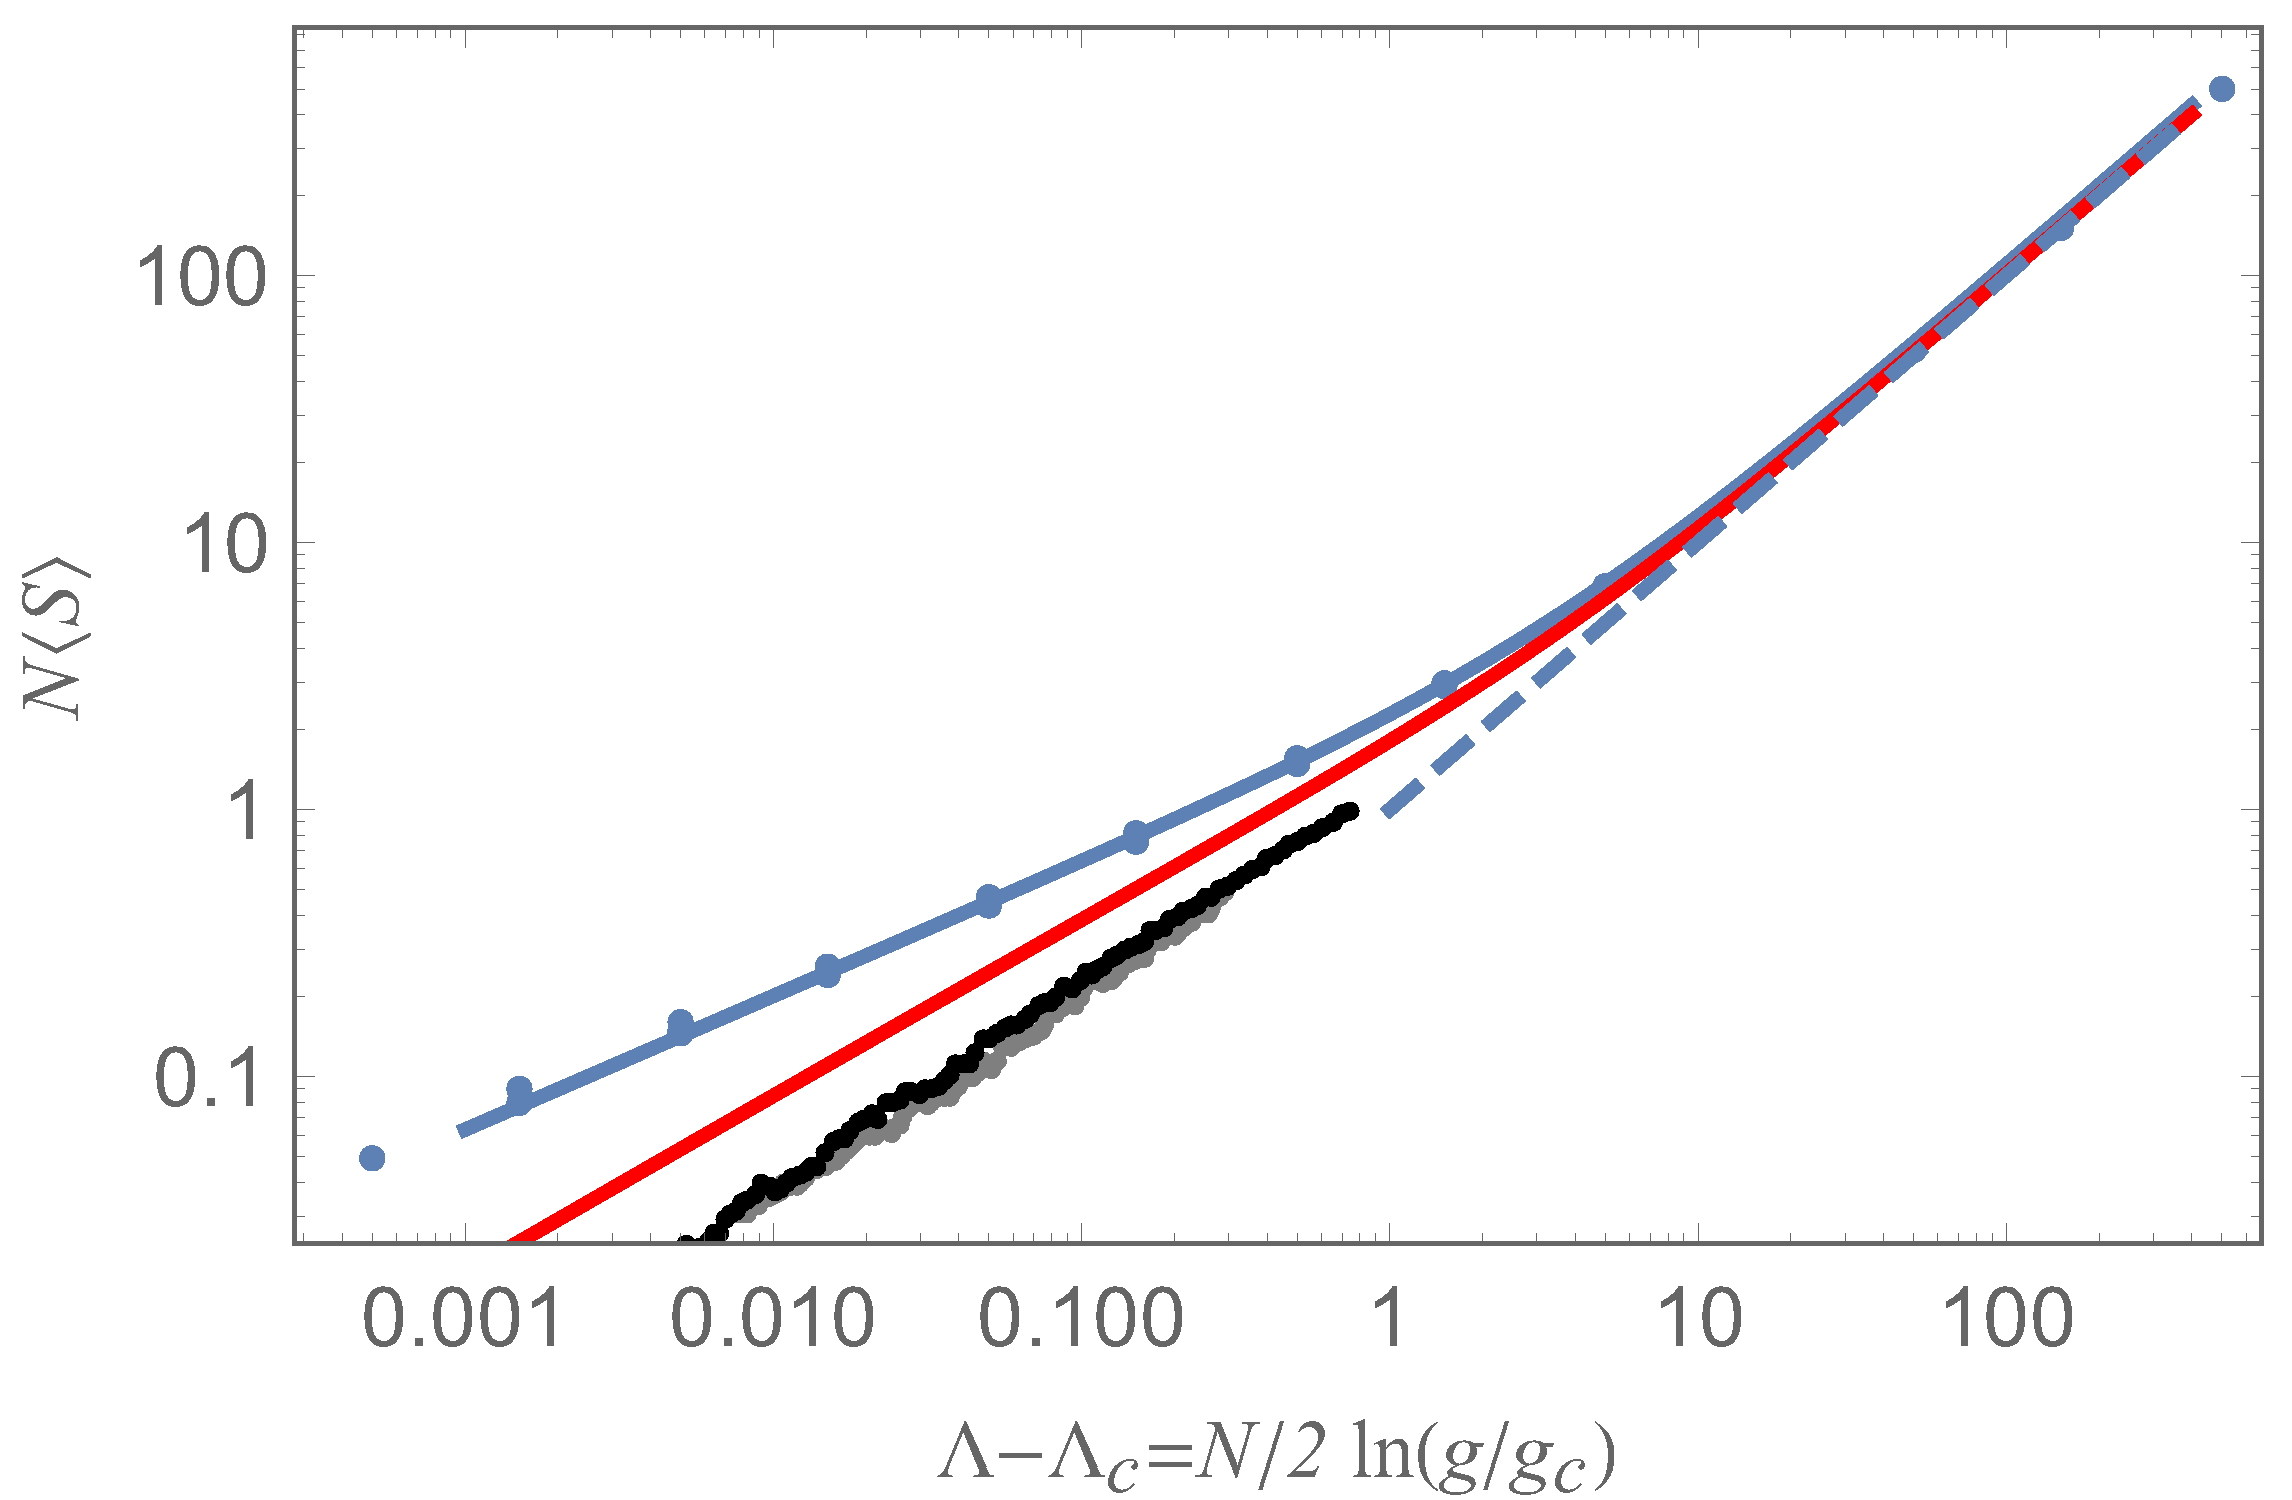
\includegraphics[width=77mm]{pngexample.png}
\caption{\small This (above) is a simple example figure and this text is the figure caption. If you are reproducing a figure from another source, make sure you reference it here and also make sure you have not copied the caption text.}
\label{fig: fig_1}
\end{figure}

%%%%%%%%%%%%%%%%%%%%%%%%%%%%%%%%%%%%%%%%%%%%%%%%%%%%%%%%%%%%%%%%%%%%%%%%%%%%%%%%%%%%
\section{Results}
This is by far the most important section of your report. It is where you will present the data you have collected during the project. There is no doubt this will be in the form of figures. A general note, you might want to split sections into subsections. This will break your report up and make it easier to read.

\begin{figure*}[]
\centering
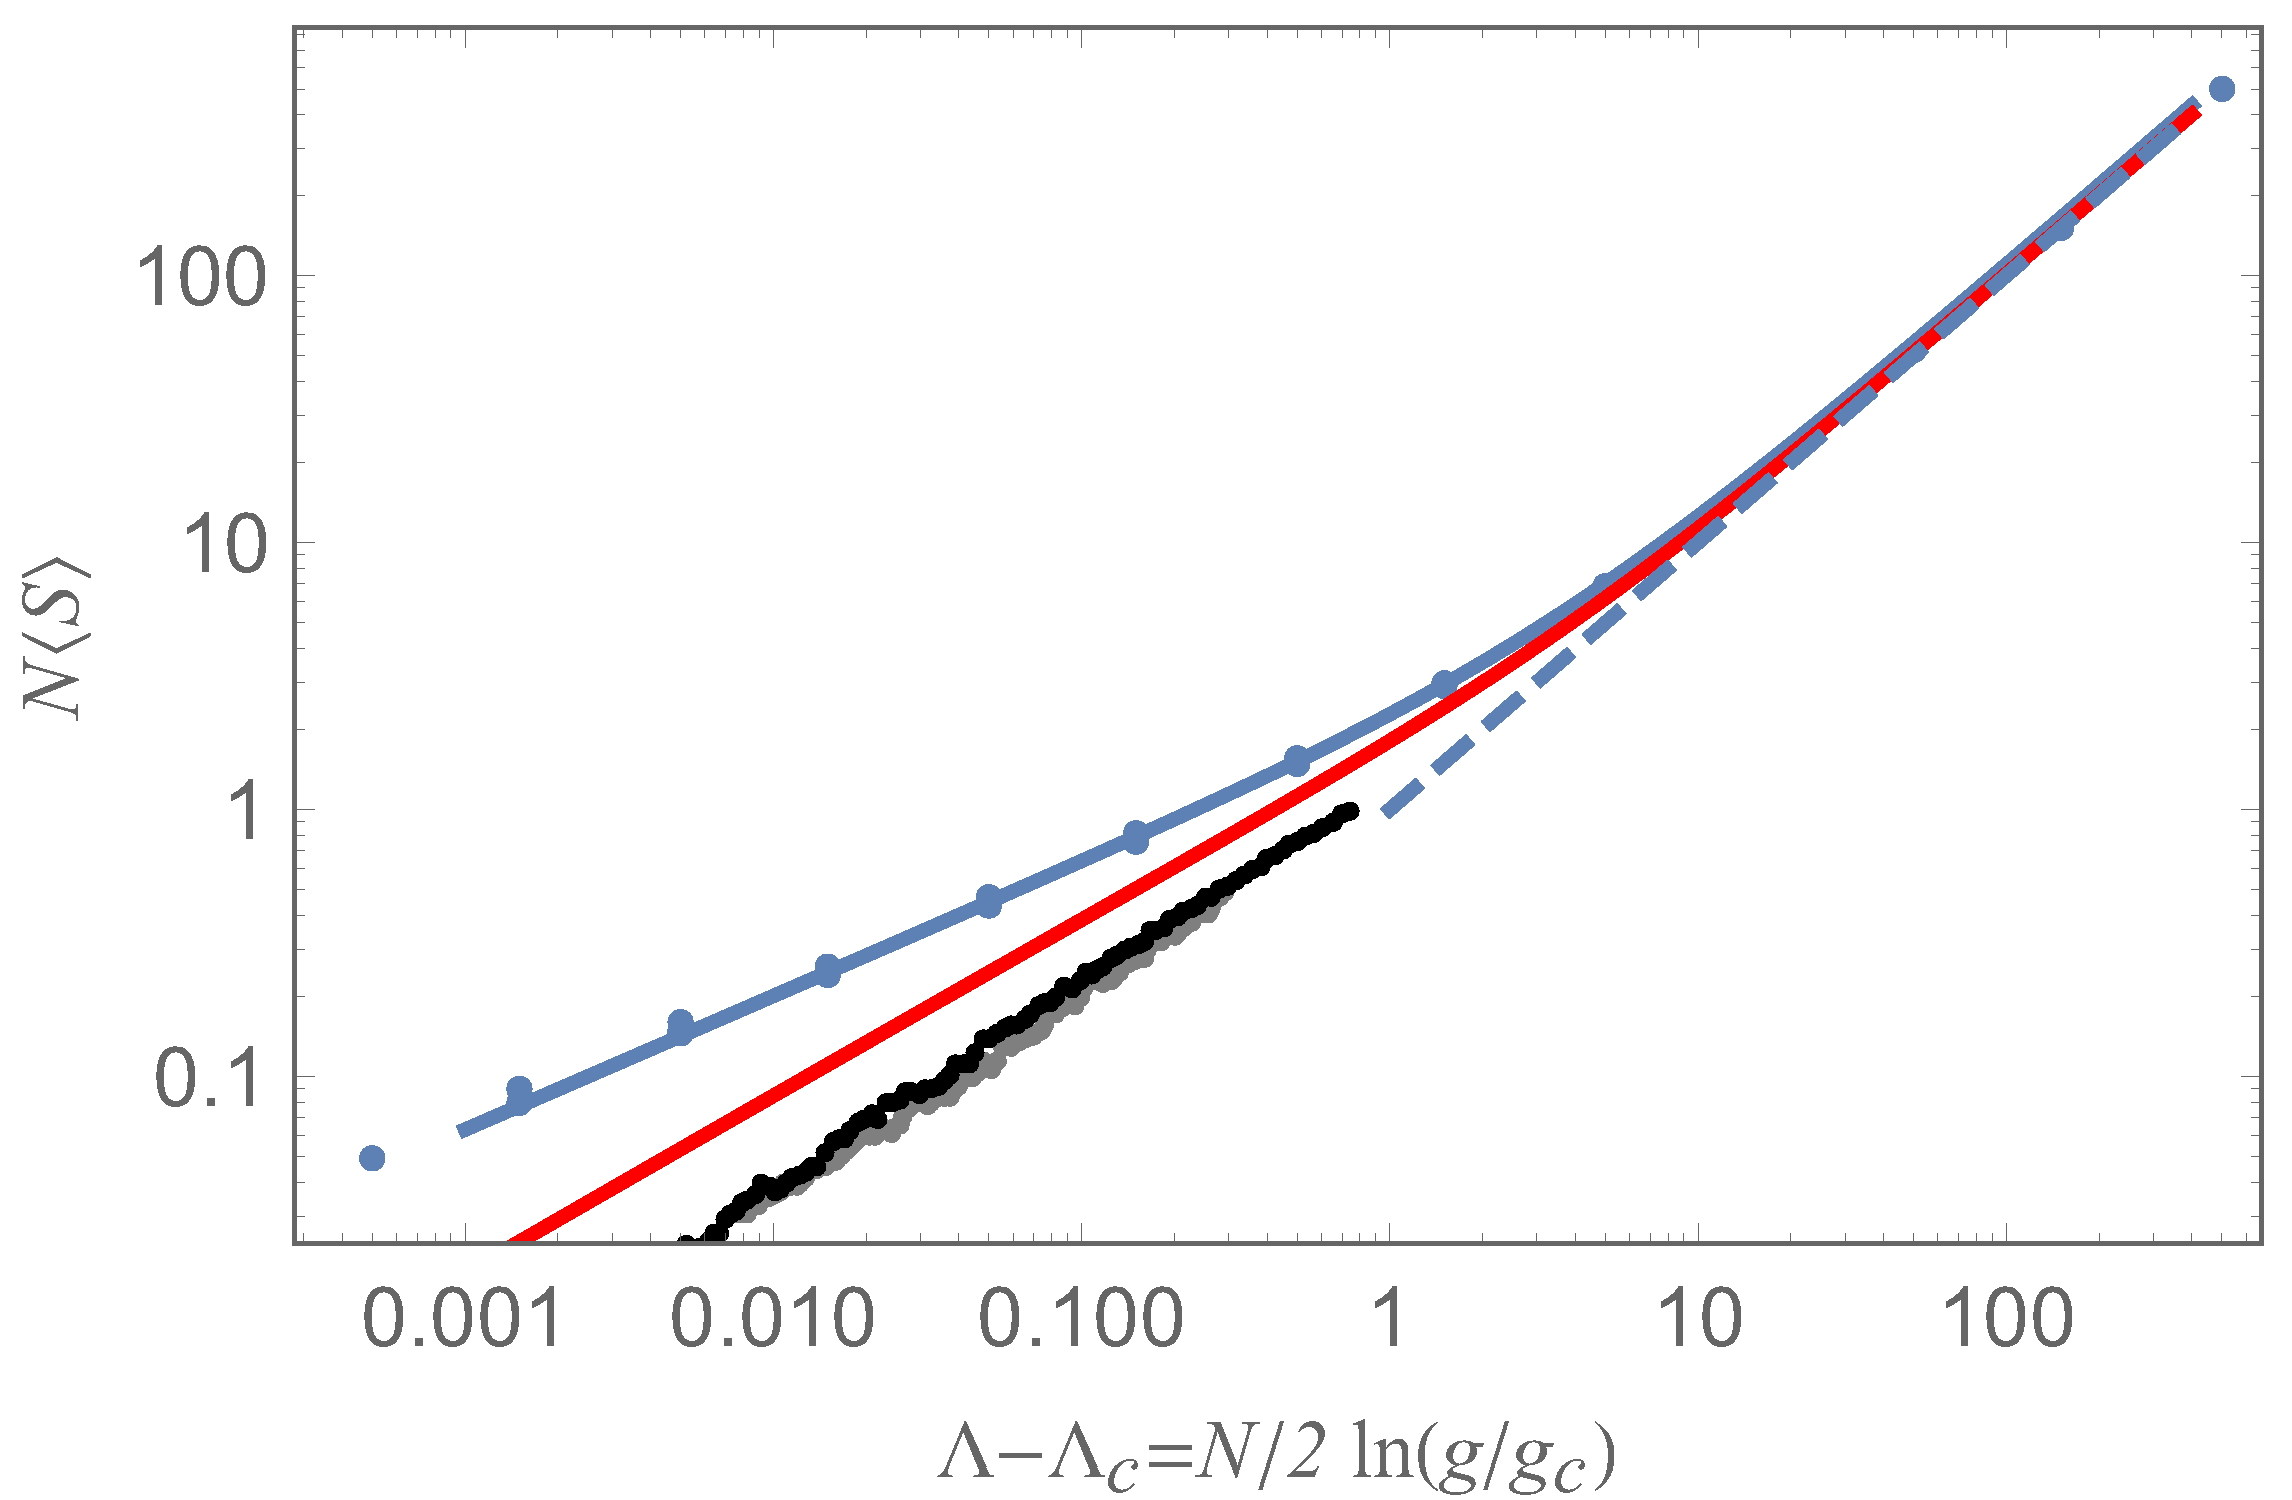
\includegraphics[width=77mm]{pngexample.png} \hspace{3mm}
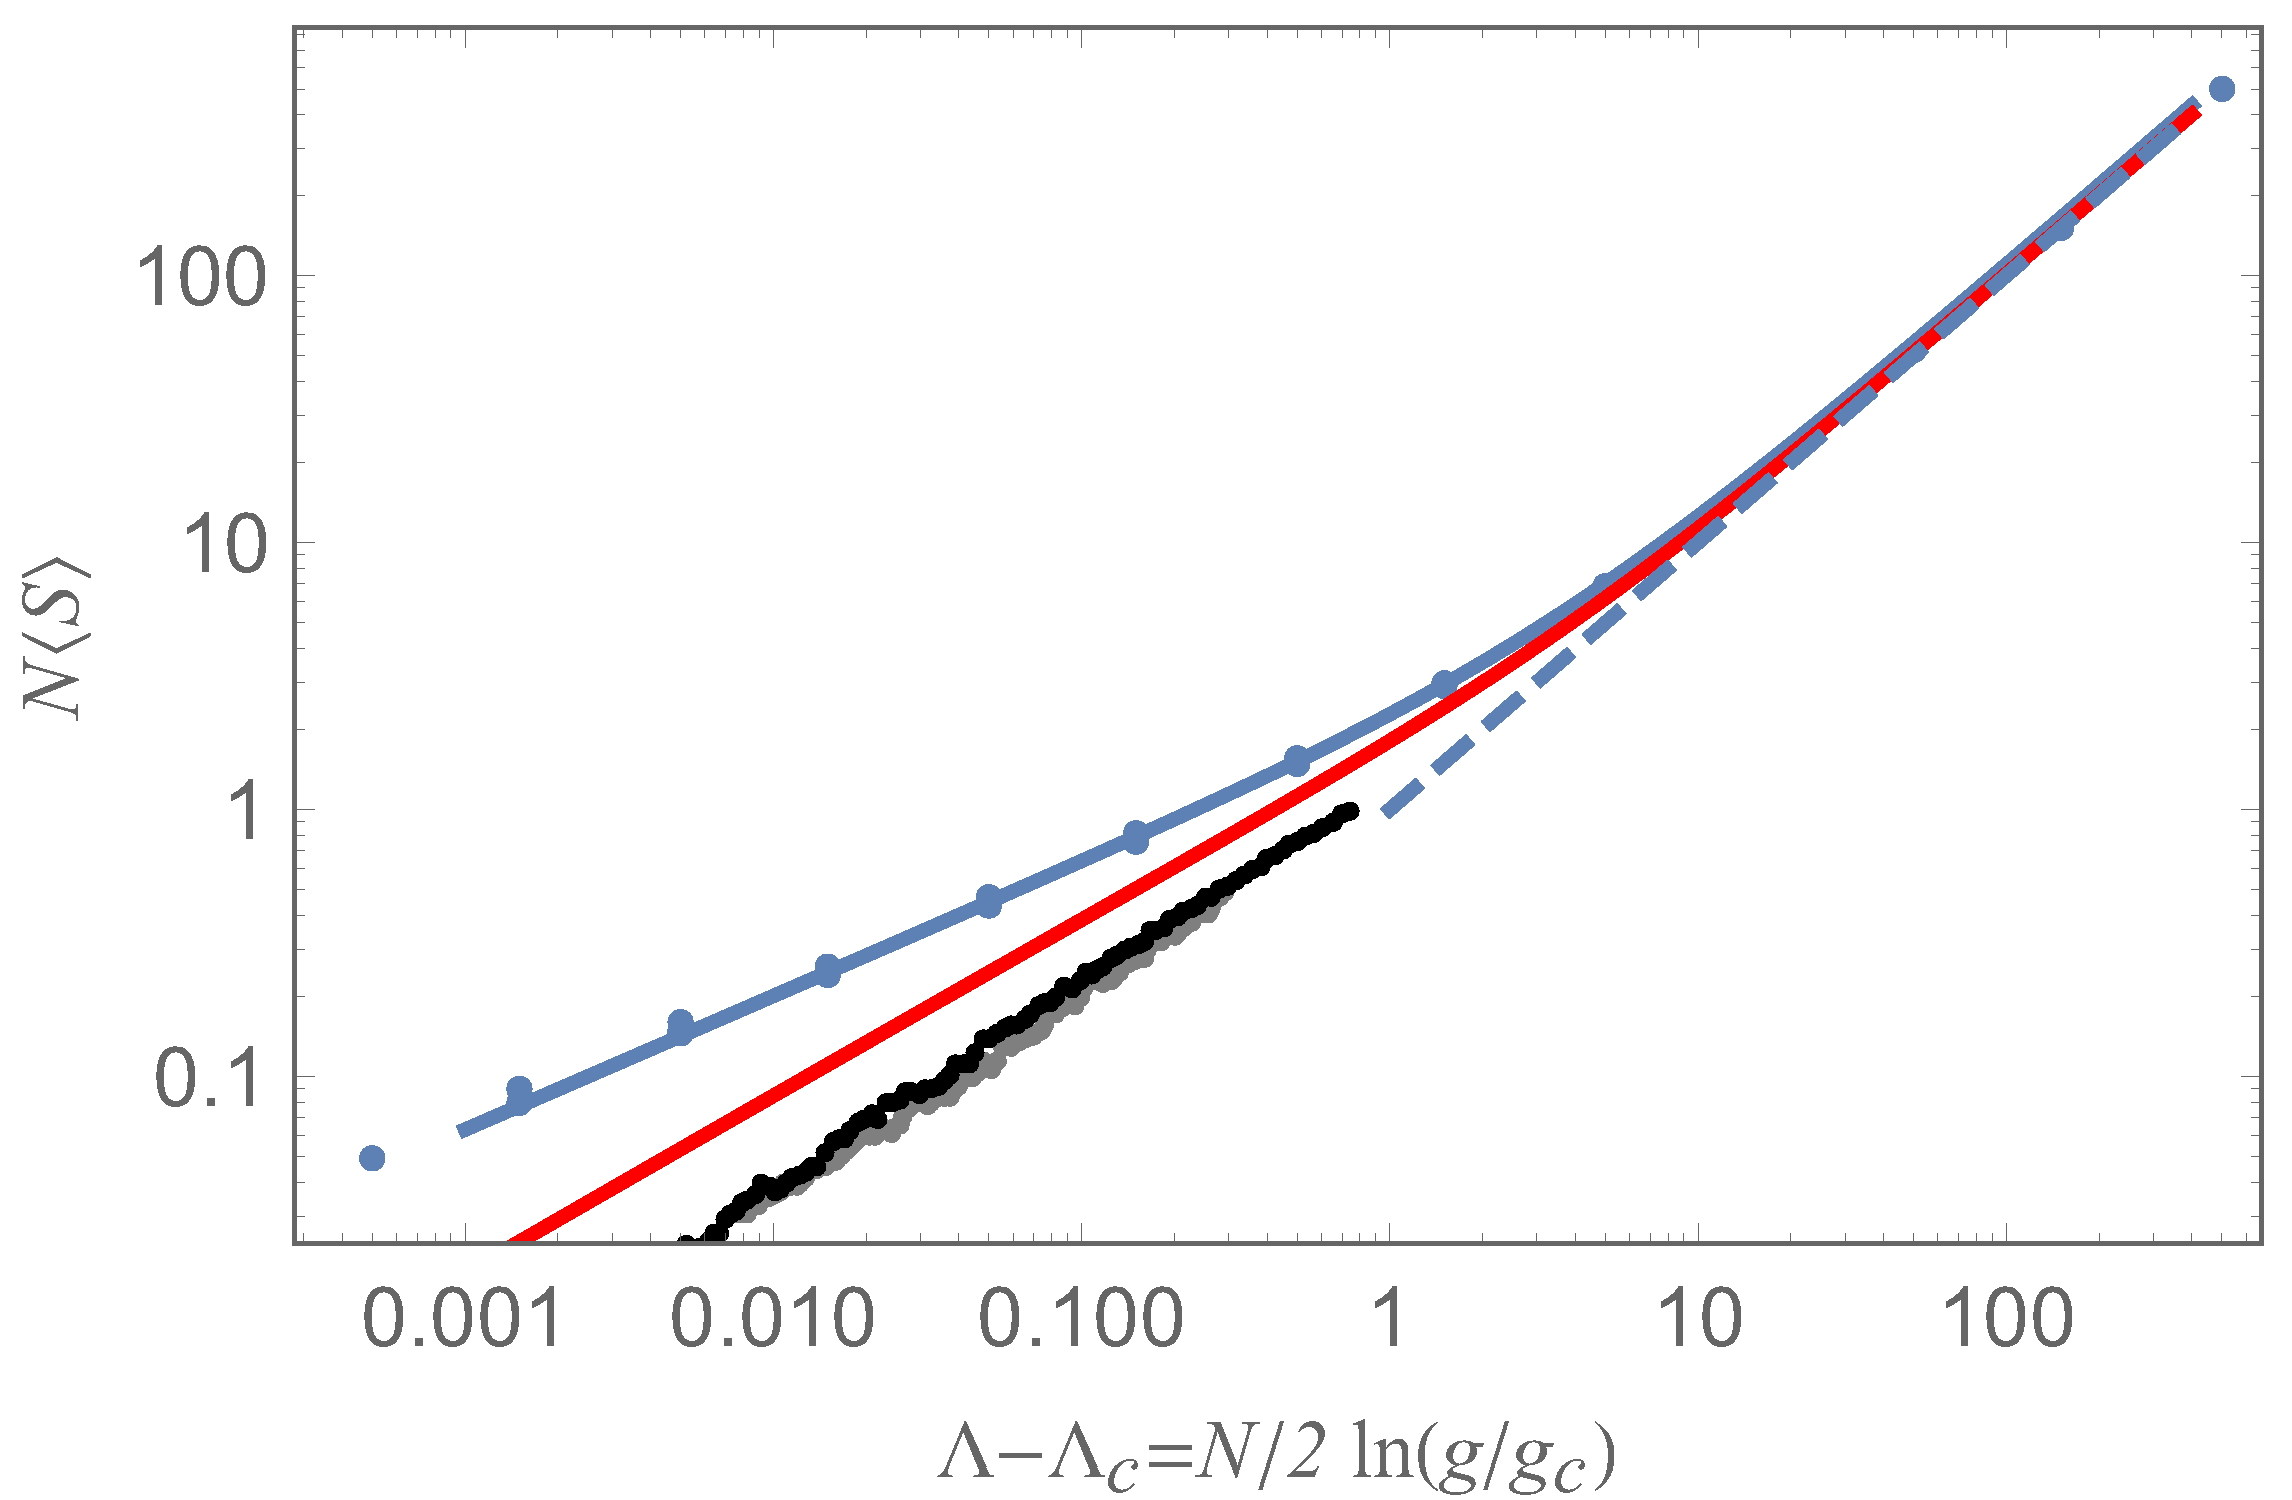
\includegraphics[width=77mm]{pngexample.png}
\caption{\small This is just an example for a wide figure.
                If you want to use *.jpg or *.pdf files
                for your figures, you need to compile with
                ``pdflatex''.}
\label{fig: fig_2}
\end{figure*}

%%%%%%%%%%%%%%%%%%%%%%%%%%%%%%%%%%%%%%%%%%%%%%%%%%%%%%%%%%%%%%%%%%%%%%%%%%%%%%%%%%%%
\subsection{Figures}
Figures should preferably occur at the top or the bottom of the page (although this is not mandatory). Such position can be achieved by using the commands \textbackslash begin\{figure\}[t or b] (See the code for an example).  


\LaTeX\ can sometimes create spaces between the figure and the caption. This can be compensated for by using \textbackslash vspace command. You might also have to refer to the figures i.e Fig. \ref{fig: fig_1}.

%%%%%%%%%%%%%%%%%%%%%%%%%%%%%%%%%%%%%%%%%%%%%%%%%%%%%%%%%%%%%%%%%%%%%%%%%%%%%%%%%%%%
\vspace{-5mm}

\subsection{More on Figures}
You may at some point have to have a large figure that spans both columns. This can be achieved by using the same environment as before but with an added asterisk (\textbackslash begin\{figure*\}). You may also use this environment to combine two related figures (see code for example).

%%%%%%%%%%%%%%%%%%%%%%%%%%%%%%%%%%%%%%%%%%%%%%%%%%%%%%%%%%%%%%%%%%%%%%%%%%%%%%%%%%%%
\subsection{Final Note on Figures}
This template uses the twocolumn environment, you can also use the multicol environment. If you opt for this please be aware that placing figures into a single column becomes a pain. This is because floats are incompatible with the multicols environment. There are a few ways around this, but I would personally suggest sticking with the twocolumn environment.

%%%%%%%%%%%%%%%%%%%%%%%%%%%%%%%%%%%%%%%%%%%%%%%%%%%%%%%%%%%%%%%%%%%%%%%%%%%%%%%%%%%%
\subsection{Tables}
\label{table}
It may be necessary to put your results in a table, this is easily done using \LaTeX\. An example of which is seen in Table \ref{tab: tab_1}.

\begin{table}[b]
\begin{tabular}{ c c c }
\hline 
 & $\mathbf{H} \parallel c$ & $\mathbf{H} \perp c$ \\ 
\hline 
$T_{\mathrm{N1}}$ (K) & 5.70(5) &  6.00(5) \\ 
$T_{\mathrm{N2}}$ (K) & 7.0(2) & 7.20(1) \\  
$\theta_{\mathrm{CW}}$ (K) & -13.7(4) & -24.5(1) \\  
$\mu_{\mathrm{eff}}$ ($\mu_{\mathrm{B}}$/Nd ion) & 10.60(2) & 10.32(4)  \\ 
\hline 
\end{tabular}
\caption{An example table}
\label{tab: tab_1}
\end{table} 


%%%%%%%%%%%%%%%%%%%%%%%%%%%%%%%%%%%%%%%%%%%%%%%%%%%%%%%%%%%%%%%%%%%%%%%%%%%%%%%%%%%%
\section{Conclusions}
You should be drawing conclusions as you discuss your results but this section acts as a summary. Many people will read the conclusion first to get a feel for the quality of the results, etc. So this can be an important section.
 
This is also my place to remind you of the length limits.  {\bf For MPhys/MMathPhys, you are recommended to aim for a length of 25 pages;}  the absolute limit is 30 pages with ONLY your bibliography (aka references list) being allowed to spill beyond that. 

{\bf For BSc you are recommended to aim for a length of 20 pages;} the absolute limit is 25 pages with ONLY your bibliography (aka references list) being allowed to spill beyond that.


%%%%%%%%%%%%%%%%%%%%%%%%%%%%%%%%%%%%%%%%%%%%%%%%%%%%%%%%%%%%%%%%%%%%%%%%%%%%%%%%%%%%

\small{
\begin{thebibliography}{99}

\setlength{\itemsep}{-2mm}

\bibitem{Paper_1} A. Author, B. Author and C. Author,
                  Journal {\bf vol}, page (year).
\bibitem{Paper_2} D. Author {\em et al.},
                  Journal {\bf vol}, page (year).
\bibitem{Paper_3} Original template by Dirk O. Gericke (2013) and edited by Daniel Brunt (2015) and Robin Ball (2018).

\end{thebibliography}
}

\end{document}